\documentclass[11pt,report]{uncdissertation}
\usepackage{lmodern}
\usepackage{amssymb,amsmath}
\usepackage{ifxetex,ifluatex}
\usepackage{fixltx2e} % provides \textsubscript
\ifnum 0\ifxetex 1\fi\ifluatex 1\fi=0 % if pdftex
  \usepackage[T1]{fontenc}
  \usepackage[utf8]{inputenc}
\else % if luatex or xelatex
  \ifxetex
    \usepackage{mathspec}
  \else
    \usepackage{fontspec}
  \fi
  \defaultfontfeatures{Ligatures=TeX,Scale=MatchLowercase}
  \newcommand{\euro}{€}
\fi
% use upquote if available, for straight quotes in verbatim environments
\IfFileExists{upquote.sty}{\usepackage{upquote}}{}
% use microtype if available
\IfFileExists{microtype.sty}{%
\usepackage{microtype}
\UseMicrotypeSet[protrusion]{basicmath} % disable protrusion for tt fonts
}{}
\usepackage[margin=1in]{geometry}
\usepackage{hyperref}
\PassOptionsToPackage{usenames,dvipsnames}{color} % color is loaded by hyperref
\hypersetup{unicode=true,
            colorlinks=true,
            linkcolor=red,
            citecolor=Blue,
            urlcolor=Blue,
            breaklinks=true}
\urlstyle{same}  % don't use monospace font for urls
\usepackage{color}
\usepackage{fancyvrb}
\newcommand{\VerbBar}{|}
\newcommand{\VERB}{\Verb[commandchars=\\\{\}]}
\DefineVerbatimEnvironment{Highlighting}{Verbatim}{commandchars=\\\{\}}
% Add ',fontsize=\small' for more characters per line
\usepackage{framed}
\definecolor{shadecolor}{RGB}{248,248,248}
\newenvironment{Shaded}{\begin{snugshade}}{\end{snugshade}}
\newcommand{\KeywordTok}[1]{\textcolor[rgb]{0.13,0.29,0.53}{\textbf{{#1}}}}
\newcommand{\DataTypeTok}[1]{\textcolor[rgb]{0.13,0.29,0.53}{{#1}}}
\newcommand{\DecValTok}[1]{\textcolor[rgb]{0.00,0.00,0.81}{{#1}}}
\newcommand{\BaseNTok}[1]{\textcolor[rgb]{0.00,0.00,0.81}{{#1}}}
\newcommand{\FloatTok}[1]{\textcolor[rgb]{0.00,0.00,0.81}{{#1}}}
\newcommand{\ConstantTok}[1]{\textcolor[rgb]{0.00,0.00,0.00}{{#1}}}
\newcommand{\CharTok}[1]{\textcolor[rgb]{0.31,0.60,0.02}{{#1}}}
\newcommand{\SpecialCharTok}[1]{\textcolor[rgb]{0.00,0.00,0.00}{{#1}}}
\newcommand{\StringTok}[1]{\textcolor[rgb]{0.31,0.60,0.02}{{#1}}}
\newcommand{\VerbatimStringTok}[1]{\textcolor[rgb]{0.31,0.60,0.02}{{#1}}}
\newcommand{\SpecialStringTok}[1]{\textcolor[rgb]{0.31,0.60,0.02}{{#1}}}
\newcommand{\ImportTok}[1]{{#1}}
\newcommand{\CommentTok}[1]{\textcolor[rgb]{0.56,0.35,0.01}{\textit{{#1}}}}
\newcommand{\DocumentationTok}[1]{\textcolor[rgb]{0.56,0.35,0.01}{\textbf{\textit{{#1}}}}}
\newcommand{\AnnotationTok}[1]{\textcolor[rgb]{0.56,0.35,0.01}{\textbf{\textit{{#1}}}}}
\newcommand{\CommentVarTok}[1]{\textcolor[rgb]{0.56,0.35,0.01}{\textbf{\textit{{#1}}}}}
\newcommand{\OtherTok}[1]{\textcolor[rgb]{0.56,0.35,0.01}{{#1}}}
\newcommand{\FunctionTok}[1]{\textcolor[rgb]{0.00,0.00,0.00}{{#1}}}
\newcommand{\VariableTok}[1]{\textcolor[rgb]{0.00,0.00,0.00}{{#1}}}
\newcommand{\ControlFlowTok}[1]{\textcolor[rgb]{0.13,0.29,0.53}{\textbf{{#1}}}}
\newcommand{\OperatorTok}[1]{\textcolor[rgb]{0.81,0.36,0.00}{\textbf{{#1}}}}
\newcommand{\BuiltInTok}[1]{{#1}}
\newcommand{\ExtensionTok}[1]{{#1}}
\newcommand{\PreprocessorTok}[1]{\textcolor[rgb]{0.56,0.35,0.01}{\textit{{#1}}}}
\newcommand{\AttributeTok}[1]{\textcolor[rgb]{0.77,0.63,0.00}{{#1}}}
\newcommand{\RegionMarkerTok}[1]{{#1}}
\newcommand{\InformationTok}[1]{\textcolor[rgb]{0.56,0.35,0.01}{\textbf{\textit{{#1}}}}}
\newcommand{\WarningTok}[1]{\textcolor[rgb]{0.56,0.35,0.01}{\textbf{\textit{{#1}}}}}
\newcommand{\AlertTok}[1]{\textcolor[rgb]{0.94,0.16,0.16}{{#1}}}
\newcommand{\ErrorTok}[1]{\textcolor[rgb]{0.64,0.00,0.00}{\textbf{{#1}}}}
\newcommand{\NormalTok}[1]{{#1}}
\usepackage{longtable,booktabs}
\usepackage{graphicx,grffile}
\makeatletter
\def\maxwidth{\ifdim\Gin@nat@width>\linewidth\linewidth\else\Gin@nat@width\fi}
\def\maxheight{\ifdim\Gin@nat@height>\textheight\textheight\else\Gin@nat@height\fi}
\makeatother
% Scale images if necessary, so that they will not overflow the page
% margins by default, and it is still possible to overwrite the defaults
% using explicit options in \includegraphics[width, height, ...]{}
\setkeys{Gin}{width=\maxwidth,height=\maxheight,keepaspectratio}
\setlength{\parindent}{0pt}
\setlength{\parskip}{6pt plus 2pt minus 1pt}
\setlength{\emergencystretch}{3em}  % prevent overfull lines
\providecommand{\tightlist}{%
  \setlength{\itemsep}{0pt}\setlength{\parskip}{0pt}}
\setcounter{secnumdepth}{5}

%%% Use protect on footnotes to avoid problems with footnotes in titles
\let\rmarkdownfootnote\footnote%
\def\footnote{\protect\rmarkdownfootnote}

%%% Change title format to be more compact
\usepackage{titling}

% Create subtitle command for use in maketitle
\newcommand{\subtitle}[1]{
  \posttitle{
    \begin{center}\large#1\end{center}
    }
}

\setlength{\droptitle}{-2em}
  \title{}
  \pretitle{\vspace{\droptitle}}
  \posttitle{}
  \author{}
  \preauthor{}\postauthor{}
  \date{}
  \predate{}\postdate{}



%Font packages
\usepackage[T1]{fontenc}
%\usepackage[latin1]{inputenc}


% List of acronyms
\usepackage{longtable}
\usepackage[acronym]{glossaries}

\usepackage{tocloft}
\usepackage{lscape}
\usepackage{tipa}

\usepackage{kvoptions}
\usepackage{setspace}
\usepackage{varwidth}
\usepackage{microtype}

\usepackage[english]{babel}


%% Math Packages %%%%%%%%%%%%%%%%%%%%%%%%%%%%%%%%%%%%%%%%%%%%
\usepackage{amsmath}
\usepackage{amsthm}
\usepackage{amsfonts}
\usepackage{bbm}
\usepackage{amssymb}
\usepackage{geometry}

%% Reduce spacing between paragraph and section title %%%%%%%
%% @todo: Put this modification in the class file itself.
\usepackage{titlesec}
\titlespacing*{\section}
{0pt}{-5pt}{0pt}
\titlespacing*{\subsection}
{0pt}{-5pt}{0pt}
\usepackage{indentfirst}   %Indents first paragraphs in every section.

%% Flush footnotes to the left
\usepackage[hang,flushmargin]{footmisc}
%% Places footnotes immediately below horizontal rule
\setlength{\footnotesep}{0pt}

%% Normal LaTeX or pdfLaTeX? %%%%%%%%%%%%%%%%%%%%%%%%%%%%%%%%
\RequirePackage{ifpdf}

% %% Packages for Graphics & Figures %%%%%%%%%%%%%%%%%%%%%%%%%%
% \ifpdf %%Inclusion of graphics via \includegraphics{file}
% 	\usepackage[pdftex]{graphicx} %%graphics in pdfLaTeX
% \else
% 	\usepackage[dvips]{graphicx} %%graphics and normal LaTeX
% \fi

% Redefines (sub)paragraphs to behave more like sections
\ifx\paragraph\undefined\else
\let\oldparagraph\paragraph
\renewcommand{\paragraph}[1]{\oldparagraph{#1}\mbox{}}
\fi
\ifx\subparagraph\undefined\else
\let\oldsubparagraph\subparagraph
\renewcommand{\subparagraph}[1]{\oldsubparagraph{#1}\mbox{}}
\fi

\begin{document}


%%%%%%%%%%%%%%%%%%%%%%%%%%%%%%%%%%%%%%%%%%%%%%%%%%%%%%%%%%%%%
%% DOCUMENT SETTINGS
%%%%%%%%%%%%%%%%%%%%%%%%%%%%%%%%%%%%%%%%%%%%%%%%%%%%%%%%%%%%%
\title{Dissertation Title}
\author{Dissertation Author}
\committee{Advisor}{Committee Member}{Committee Member}{Committee Member}{Committee Member}
\date{January 1, 1970}

\abstract{this is good stuff}

\dedication{To someone}

\pagestyle{plain}

\frontmatter{}


\maketitlepg
\makecopyrightpg
\makeabstractpg
\makededicationpg

\chapter*{Acknowledgements}
Insert your acknowledgements here. 

This should be one page maximum, and is single-spaced by default.



% The graduate school requires that entries are double spaced.
% They also require that multiple lines in a single entry are single spaced.
% This achieves that by setting \baselineskip (the space between lines)
% and \parskip (the additional space between paragraphs) directly, then restoring them
%
% @todo: Find a more elegant way of achieving this

% Establish original spacings

\newlength{\oldbaselineskip}
\setlength{\oldbaselineskip}{\the\baselineskip}
\newlength{\oldparskip}
\setlength{\oldparskip}{\the\parskip}


\newpage

% Set spacings for these sections
\setlength{\baselineskip}{0.5\oldbaselineskip}
\setlength{\parskip}{0.5\oldbaselineskip}


\tableofcontents

\newpage

\listoffigures

\newpage

\listoftables


% Restore original spacings
\setlength{\baselineskip}{1.0\oldbaselineskip}
\setlength{\parskip}{1.0\oldparskip}

\listofabbreviations

\mainmatter

\chapter{Introduction - Markdown and \LaTeX\label{intro}}

This is a piecemeal rendition of the University of Arizona thesis class
(\texttt{uathesis}) reworked to be compatible with \texttt{Rmarkdown}.
The majority of the heavy lifting was already done by colleagues in the
Department of Planetary Sciences at the U of A (see the
\texttt{uathesis.cls} file for more information). In essence all I have
done is include the proper adjustments so that it plays nicely with
\texttt{knitr}. As of now (Sat Sep 10 09:18:17 2016), knitr and R are
fully functional. That said, some other issues still remain.

\section{\texorpdfstring{Issues\label{issues}}{Issues}}\label{issues}

\begin{itemize}
\tightlist
\item
  Knitr captions

  \begin{itemize}
  \tightlist
  \item
    include captions from knitr call
  \item
    include figure in LOF from knitr call
  \end{itemize}
\end{itemize}

\section{Basic structure}\label{basic-structure}

The basic structure of the thesis package has been cleaned up
significantly. There are now two folders inside the main directory:
\textbf{includes} and \textbf{sections}. The \texttt{includes} folder
contains most of the under the hood files that you will generally edit
one time to set up the project metadata (i.e.~the title, committee
members, etc.), but also includes .bib files and figures. The
\texttt{sections} folder is where the chapters of the dissertation live.
Each chapter is its own .Rmd file. You will write you chapters in these
files and compile the master document. This folder is home to the other
less important (but required) sections (i.e.~acknowledgments,
dedications, abstracts and appendices).\footnote{All of these files are
  imported into the final pdf in the \texttt{master.Rmd} file via
  \texttt{knitr} or specific commands written for the \texttt{uathesis}
  class.} The underlying engine is \LaTeX. To generate the dissertation
pdf, compile the \texttt{master.Rmd} file in your favorite text editor.

\section{\texorpdfstring{Sections\label{sections}}{Sections}}\label{sections}

You can use either markdown or \LaTeX~to create sections in the document
(see general markdown syntax for more information). In both cases,
cross-referencing figure, tables, sections, chapters, etc. can only be
done if a \texttt{label\{\}} is created. For example, this is section
\ref{sections}. I generated that number by first labeling the
section\ldots  

\begin{verbatim}
# Sections\label{sections}
\end{verbatim}

and then by typing\ldots  

\begin{verbatim}
\ref{sections}
\end{verbatim}

It is helpful to use this with figures and tables. Like, for Figure
\ref{fig:firstfig} and Table \ref{sampletable} below.

\subsection{Subsections}\label{subsections}

You can use hashtags or the \texttt{\textbackslash{}subsection\{\}}
command to create a subsection.

\subsubsection{Subsubsections}\label{subsubsections}

These have been fixed. You can use
\texttt{\textbackslash{}subsubsection\{\}} or 3 hashtags.

\paragraph{Subsubsubsections}

If you really need to go this deep, I suggest using the
\texttt{\textbackslash{}paragraph\{\}} command.

\section{\texorpdfstring{Math
Example\label{math}}{Math Example}}\label{math-example}

Equations can be rendered beautifully by using the \texttt{equation}
environment.

\begin{equation}
    y = mx + b
\end{equation}

But, old school math works too!

\[ \begin{aligned} y &= \beta_0 + \beta_1 + x_1 + \epsilon \end{aligned} \]

But putting it inside the \texttt{equation} environment will number it
(as in the first example), and has the added advantage of centering
automatically as well.

\begin{equation}
    y = \beta_0 + \beta_1 + x_1 + \epsilon
\end{equation}

\section{\texorpdfstring{How to cite your
references\label{ref_citation}}{How to cite your references}}\label{how-to-cite-your-references}

One relevant difference from the previous iteration of this package is
that it now uses \texttt{Rmarkdown/pandoc} to render citations. This is
a work is progress, but for now you can reference by using the standard
\texttt{{[}@citekey{]}} method. For example, citations are cool {[}1{]}.
For inline citations, remove the brackets (i.e. \texttt{@articletwo}).
As in {[}2{]} said many things.

\section{\texorpdfstring{Graphics\label{graphics}}{Graphics}}\label{graphics}

This took a little cajoling, but the figures are now working. They are
automatically included in the list of figures and you can use the
brackets in the caption to establish a different LOF caption (separate
from the one you see below.).

\begin{figure}[h]
    \centering
    \caption[Example figure]{Here is a screeny of the sections folder.}
    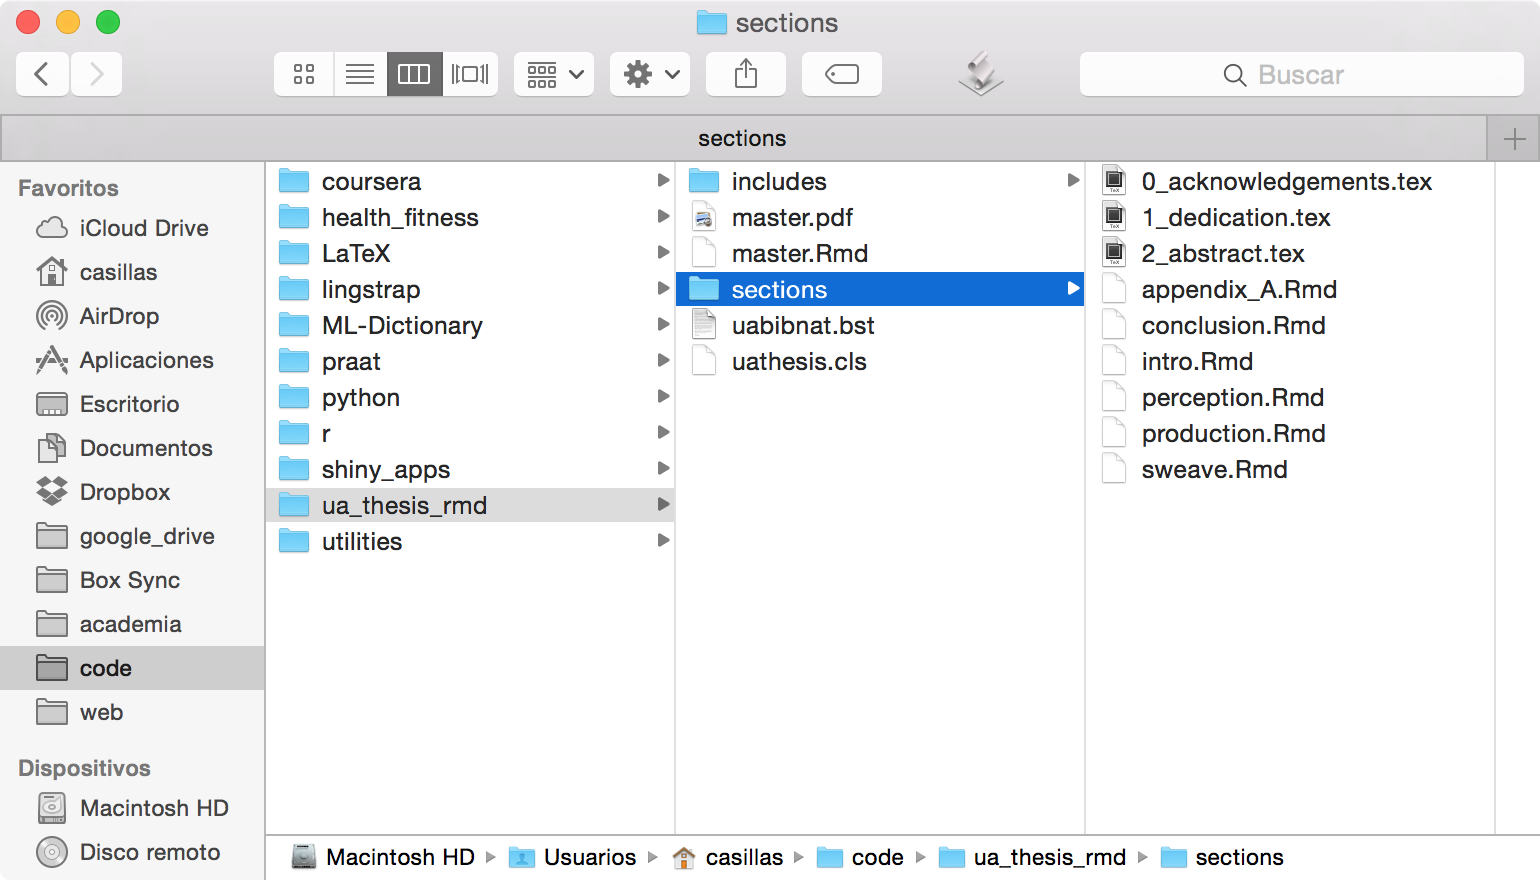
\includegraphics[width=.75\textwidth]{./includes/figures/ex.png}
    \label{fig:firstfig}
\end{figure}

One thing to remember is that when including images the home directory
is always that of the \texttt{master.Rmd} document. Therefore, it is
necessary to establish the path to the img file from there. Here is the
code used to produce the above figure:

\begin{verbatim}
\begin{figure}[h]
    \centering
    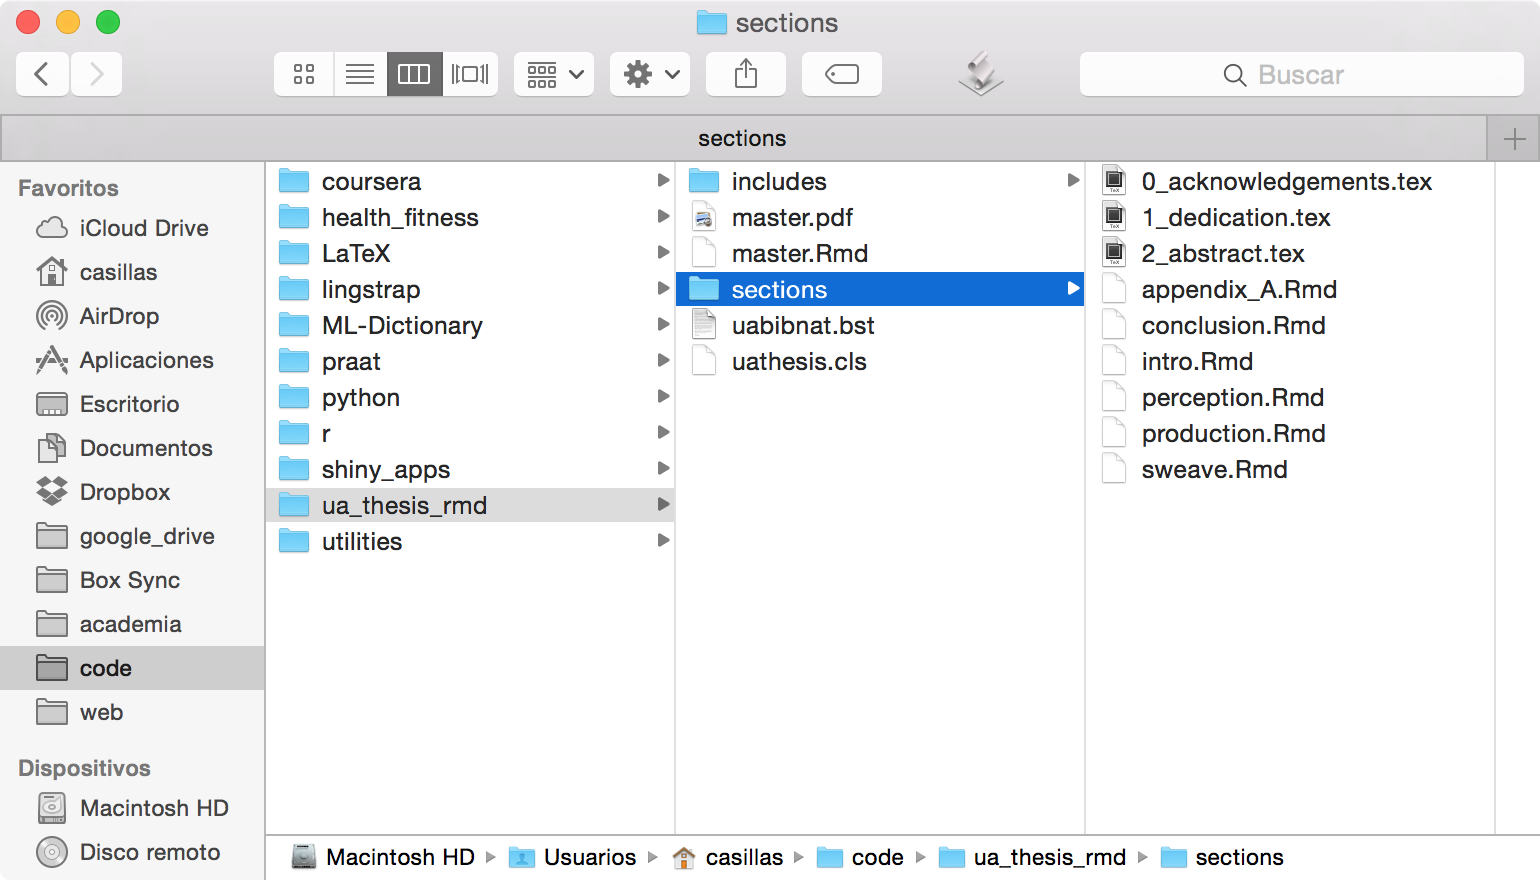
\includegraphics[width=.75\textwidth]{./includes/figures/ex.png}
    \caption[Example figure]{Here is a screeny of the sections folder.}
    \label{fig:firstfig}
\end{figure}
\end{verbatim}

\chapter{More \LaTeX\label{exp1}}

\section{\texorpdfstring{Tables\label{tables}}{Tables}}\label{tables}

Tables work the same way as before\ldots

\begin{table}[h]
  \begin{center}
  \caption[Another table caption here]{Another table caption (to appear with the actual table). \label{table1}}
  \vspace{0.3in}
    \begin{tabular}{ccc}
      \hline 
      \hline
      Col A & Col B & Col C \\
      \hline
      1     & 2     & 3     \\
      4     & 5     & 6     \\
      \hline
    \end{tabular}
  \end{center}
\end{table}

They can be rendered in markdown now as well (and can include r code),
but I don't recommend this combination (for now)\ldots

\begin{longtable}[c]{@{}lll@{}}
\toprule
Col 1 & Col 2 & col 3\tabularnewline
\midrule
\endhead
4 & plus & 8\tabularnewline
equals & 12 & nice!\tabularnewline
\bottomrule
\end{longtable}

On the next page is a sample table, placed on the page by itself.
Sometimes tables can be wider than they are tall, and you may need to
rotate the table by \(90^{\circ}\) to make it fit better on a page by
itself. To do that you can use the lscape package. To use it, wrap the
table commands in a begin and end landscape command and that table will
be properly rotated.

\begin{landscape}
\begin{table}[p!]
  \begin{center}
  \caption[Short table caption here]{Sample table caption (to appear with the actual table). \label{sampletable}}
  \vspace{0.3in}
    \begin{tabular}{ccc}
      \hline 
      \hline
      Col A & Col B & Col C \\
      \hline
      1     & 2     & 3     \\
      4     & 5     & 6     \\
      \hline
    \end{tabular}
  \end{center}
\end{table}
\end{landscape}

Note that the \verb=\caption= command can have a short and a long
version inside a table environment, just like inside a figure
environment (see \ref{graphics}).

\section{\texorpdfstring{TIPA\label{using IPA}}{TIPA}}\label{tipa}

You can include IPA characters via the \texttt{TIPA} package. Here is an
example:

\textipa{[Sip]-[SIp]} - Looks good.

\chapter{Using R\label{rcode}}

\section{Basic math}\label{basic-math}

Here are some simple math examples

\begin{Shaded}
\begin{Highlighting}[]
\DecValTok{24} \NormalTok{-}\StringTok{ }\DecValTok{23}
\end{Highlighting}
\end{Shaded}

\begin{verbatim}
## [1] 1
\end{verbatim}

\begin{Shaded}
\begin{Highlighting}[]
\DecValTok{2345} \NormalTok{*}\StringTok{ }\DecValTok{23}
\end{Highlighting}
\end{Shaded}

\begin{verbatim}
## [1] 53935
\end{verbatim}

\section{Inline expressions}\label{inline-expressions}

You can use inline r expressions like 2 plus 2 = 0

\section{Run models}\label{run-models}

\begin{Shaded}
\begin{Highlighting}[]
\KeywordTok{library}\NormalTok{(xtable); }\KeywordTok{library}\NormalTok{(dplyr)}
\NormalTok{mtcars %>%}
\StringTok{  }\KeywordTok{glm}\NormalTok{(vs ~}\StringTok{ }\NormalTok{mpg, }\DataTypeTok{data =} \NormalTok{., }\DataTypeTok{family =} \StringTok{"binomial"}\NormalTok{) %>%}
\StringTok{  }\KeywordTok{xtable}\NormalTok{(., }\DataTypeTok{type =} \StringTok{"latex"}\NormalTok{) %>%}
\StringTok{  }\KeywordTok{print}\NormalTok{(}\DataTypeTok{comment =} \OtherTok{FALSE}\NormalTok{)}
\end{Highlighting}
\end{Shaded}

\begin{table}[ht]
\centering
\begin{tabular}{rrrrr}
  \hline
 & Estimate & Std. Error & z value & Pr($>$$|$z$|$) \\ 
  \hline
(Intercept) & -8.8331 & 3.1623 & -2.79 & 0.0052 \\ 
  mpg & 0.4304 & 0.1584 & 2.72 & 0.0066 \\ 
   \hline
\end{tabular}
\end{table}

\section{Plots}\label{plots}

And you can generate plots directly from this file as well.

\begin{Shaded}
\begin{Highlighting}[]
\KeywordTok{library}\NormalTok{(ggplot2)}
\KeywordTok{ggplot}\NormalTok{(mtcars, }\KeywordTok{aes}\NormalTok{(}\DataTypeTok{x =} \NormalTok{mpg, }\DataTypeTok{y =} \NormalTok{vs)) +}\StringTok{ }
\KeywordTok{geom_point}\NormalTok{() +}\StringTok{ }
\KeywordTok{geom_smooth}\NormalTok{(}\DataTypeTok{method =} \StringTok{"glm"}\NormalTok{, }\DataTypeTok{method.args=}\KeywordTok{list}\NormalTok{(}\DataTypeTok{family=}\StringTok{"binomial"}\NormalTok{))}
\end{Highlighting}
\end{Shaded}

\includegraphics{dissertation_files/figure-latex/unnamed-chunk-9-1.pdf}

\chapter{Sourcing .R files\label{conclusion}}

\section{Import scripts}\label{import-scripts}

We can use the following command to import an r script:

\begin{Shaded}
\begin{Highlighting}[]
\KeywordTok{library}\NormalTok{(knitr)}
\KeywordTok{read_chunk}\NormalTok{(}\StringTok{'../includes/scripts/test.R'}\NormalTok{)}
\end{Highlighting}
\end{Shaded}

\section{Call chunks}\label{call-chunks}

\begin{Shaded}
\begin{Highlighting}[]
\KeywordTok{library}\NormalTok{(dplyr); }\KeywordTok{library}\NormalTok{(lingStuff)}
\end{Highlighting}
\end{Shaded}

\begin{Shaded}
\begin{Highlighting}[]
\CommentTok{# Generate data}
\KeywordTok{set.seed}\NormalTok{(}\DecValTok{1}\NormalTok{)}
\NormalTok{vot =}\StringTok{ }\KeywordTok{rnorm}\NormalTok{(}\DecValTok{20}\NormalTok{, }\DecValTok{15}\NormalTok{, }\DecValTok{5}\NormalTok{)}
\NormalTok{vot =}\StringTok{ }\KeywordTok{sort}\NormalTok{(vot)}
\NormalTok{phon =}\StringTok{ }\KeywordTok{c}\NormalTok{(}\DecValTok{0}\NormalTok{,}\DecValTok{1}\NormalTok{,}\DecValTok{0}\NormalTok{,}\DecValTok{0}\NormalTok{,}\DecValTok{0}\NormalTok{,}\DecValTok{0}\NormalTok{,}\DecValTok{0}\NormalTok{,}\DecValTok{1}\NormalTok{,}\DecValTok{0}\NormalTok{,}\DecValTok{1}\NormalTok{,}\DecValTok{0}\NormalTok{,}\DecValTok{1}\NormalTok{,}\DecValTok{0}\NormalTok{,}\DecValTok{1}\NormalTok{,}\DecValTok{1}\NormalTok{,}\DecValTok{1}\NormalTok{,}\DecValTok{1}\NormalTok{,}\DecValTok{1}\NormalTok{,}\DecValTok{1}\NormalTok{,}\DecValTok{1}\NormalTok{)}
\NormalTok{df =}\StringTok{ }\KeywordTok{as.data.frame}\NormalTok{(}\KeywordTok{cbind}\NormalTok{(vot, phon))}
\end{Highlighting}
\end{Shaded}

\begin{Shaded}
\begin{Highlighting}[]
\CommentTok{# Fit model}
\NormalTok{glm <-}\StringTok{ }\KeywordTok{glm}\NormalTok{(phon ~}\StringTok{ }\NormalTok{vot, }\DataTypeTok{data =} \NormalTok{df, }\DataTypeTok{family =} \StringTok{"binomial"}\NormalTok{)}
\end{Highlighting}
\end{Shaded}

\begin{Shaded}
\begin{Highlighting}[]
\CommentTok{# Get crossover point}

\KeywordTok{crossOver}\NormalTok{(glm)}
\end{Highlighting}
\end{Shaded}

\begin{verbatim}
## [1] 15.53595
\end{verbatim}

. Good. Let's plot it --\textgreater{}

\begin{Shaded}
\begin{Highlighting}[]
\CommentTok{# Plot regression with crossover point}

\KeywordTok{plot}\NormalTok{(df$vot, df$phon, }\DataTypeTok{xlab =} \StringTok{"vot"}\NormalTok{, }\DataTypeTok{ylab =} \StringTok{"phon"}\NormalTok{,}
     \DataTypeTok{pch =} \DecValTok{16}\NormalTok{, }\DataTypeTok{col =} \KeywordTok{rgb}\NormalTok{(}\DecValTok{0}\NormalTok{, }\DecValTok{0}\NormalTok{, }\DecValTok{204}\NormalTok{, }\DecValTok{102}\NormalTok{, }\DataTypeTok{maxColorValue =} \DecValTok{255}\NormalTok{))}
\KeywordTok{curve}\NormalTok{(}\KeywordTok{predict}\NormalTok{(glm, }\KeywordTok{data.frame}\NormalTok{(}\DataTypeTok{vot =} \NormalTok{x), }\DataTypeTok{type =} \StringTok{"resp"}\NormalTok{), }\DataTypeTok{add =} \OtherTok{TRUE}\NormalTok{)}
\KeywordTok{points}\NormalTok{(vot, }\KeywordTok{fitted}\NormalTok{(glm), }\DataTypeTok{pch =} \DecValTok{20}\NormalTok{)}
\KeywordTok{abline}\NormalTok{(}\DataTypeTok{v =} \KeywordTok{crossOver}\NormalTok{(glm), }\DataTypeTok{lty =} \DecValTok{2}\NormalTok{, }\DataTypeTok{lwd =} \FloatTok{0.75}\NormalTok{)}
\KeywordTok{abline}\NormalTok{(}\DataTypeTok{h =} \FloatTok{0.5}\NormalTok{, }\DataTypeTok{v =} \DecValTok{0}\NormalTok{)}
\end{Highlighting}
\end{Shaded}

\begin{figure}[htbp]
\centering
\includegraphics{dissertation_files/figure-latex/plot-1.pdf}
\caption{This is the caption}
\end{figure}

\appendix

\chapter{Sample Appendix\label{apndxA}}

Stuff\ldots{}..

\chapter{Another Appendix\label{apndxB}}

Lorem ipsum dolor sit amet, consectetur adipisicing elit, sed do eiusmod
tempor incididunt ut labore et dolore magna aliqua. Ut enim ad minim
veniam, quis nostrud exercitation ullamco laboris nisi ut aliquip ex ea
commodo consequat. Duis aute irure dolor in reprehenderit in voluptate
velit esse cillum dolore eu fugiat nulla pariatur. Excepteur sint
occaecat cupidatat non proident, sunt in culpa qui officia deserunt
mollit anim id est laborum.

\setlength{\parindent}{-0.2in} \setlength{\leftskip}{0.2in}
\setlength{\parskip}{8pt}

\increferences{sections/references}

\hypertarget{refs}{}
\hypertarget{ref-article}{}
{[}1{]} Author F, Author S, Author T. Random article about some stuff.
Random Journal 2002;666:1--20.

\hypertarget{ref-articletwo}{}
{[}2{]} Author F, Author S, Author T. Some more random stuff. Random
Journal 2015;675:1--20.

\end{document}
